\documentclass[conference]{IEEEtran}
\IEEEoverridecommandlockouts
% The preceding line is only needed to identify funding in the first footnote. If that is unneeded, please comment it out.
\usepackage{cite}
\usepackage{amsmath,amssymb,amsfonts}
\usepackage{algorithmic}
\usepackage{graphicx}
\usepackage{textcomp}
\usepackage{xcolor}
\usepackage{listings}
\def\BibTeX{{\rm B\kern-.05em{\sc i\kern-.025em b}\kern-.08em
    T\kern-.1667em\lower.7ex\hbox{E}\kern-.125emX}}

\definecolor{keywords}{RGB}{255,0,90}
\definecolor{comments}{RGB}{0,0,113}
\definecolor{red}{RGB}{160,0,0}
\definecolor{green}{RGB}{0,150,0}
\begin{document}

\lstset{language=Python, 
        basicstyle=\ttfamily\small, 
        keywordstyle=\color{keywords},
        commentstyle=\color{comments},
                stringstyle=\color{red},
        showstringspaces=false,
        identifierstyle=\color{green},
        keywords=[2]{pow},
        keywordstyle=[2]{\color{orange}},
}
\lstset{frame=lines}
%\lstset{caption={Insert code directly in your document}}
\lstset{label={lst:code_direct}}
\lstset{basicstyle=\footnotesize}


\title{Conference Paper Title*\\
{\footnotesize \textsuperscript{*}Note: Sub-titles are not captured in Xplore and
should not be used}
\thanks{Identify applicable funding agency here. If none, delete this.}
}

\author{\IEEEauthorblockN{1\textsuperscript{st} Given Name Surname}
\IEEEauthorblockA{\textit{dept. name of organization (of Aff.)} \\
\textit{name of organization (of Aff.)}\\
City, Country \\
email address or ORCID}
\and
\IEEEauthorblockN{2\textsuperscript{nd} Given Name Surname}
\IEEEauthorblockA{\textit{dept. name of organization (of Aff.)} \\
\textit{name of organization (of Aff.)}\\
City, Country \\
email address or ORCID}
\and
\IEEEauthorblockN{3\textsuperscript{rd} Given Name Surname}
\IEEEauthorblockA{\textit{dept. name of organization (of Aff.)} \\
\textit{name of organization (of Aff.)}\\
City, Country \\
email address or ORCID}
\and
\IEEEauthorblockN{4\textsuperscript{th} Given Name Surname}
\IEEEauthorblockA{\textit{dept. name of organization (of Aff.)} \\
\textit{name of organization (of Aff.)}\\
City, Country \\
email address or ORCID}
\and
\IEEEauthorblockN{5\textsuperscript{th} Given Name Surname}
\IEEEauthorblockA{\textit{dept. name of organization (of Aff.)} \\
\textit{name of organization (of Aff.)}\\
City, Country \\
email address or ORCID}
\and
\IEEEauthorblockN{6\textsuperscript{th} Given Name Surname}
\IEEEauthorblockA{\textit{dept. name of organization (of Aff.)} \\
\textit{name of organization (of Aff.)}\\
City, Country \\
email address or ORCID}
}

\maketitle

\begin{abstract}
This document is a model and instructions for \LaTeX.
This and the IEEEtran.cls file define the components of your paper [title, text, heads, etc.]. *CRITICAL: Do Not Use Symbols, Special Characters, Footnotes, 
or Math in Paper Title or Abstract.
\end{abstract}

\begin{IEEEkeywords}
component, formatting, style, styling, insert
\end{IEEEkeywords}

\section{Einleitung}


Im laufe der Jahre, findet MQTT vielseitigen Einsatz, für Sensordaten, klassische Nachrichten, Aktienkurse oder Kurzmitteilungen bei der Facebook Mobil App.
Dies weckt Interesse bei vielen Nutzern,sich mit dem Thema MQTT vertraut zu machen.

MQTT ist ein Client-Server-Protokoll.
Clients senden dem Server (Broker)nach Verbindungsaufbau Nachrichten mit einem Topic,welches die versendeten Nachrichten strukturiert. 
Zum Beispiel Haus/Wohnzimmer/Sofa.

So hat sich unsere Gruppe die Aufgabe gestellt, das MQTT Projekt MQTTexercise2021 zu programmieren und so Kenntnisse zum Thema Mqtt zu sammeln.

In dem Projekt haben wir uns die Aufgabe gestellt, einen Server zu Programmieren der Nachrichten von anderen Clients (User, Services, Taxi) empfängt und Nachrichten versenden kann.

\subsection{Aufgaben}

Server: Registriert alle Clients, verteilt IDS, übermittelt Nachrichten, 
erhält Nachrichten, leitet/organisiert den Ablaufplan.

User: Anmelden beim Server, order Fahrzeug, sendet Koordinaten, Fahrzeug kommt, wird zum Zielort gebracht, setzt Car free

Taxi: Anmeldung Server, fährt zu den Koordinaten, übermittelt Koordinaten, übermittelt Nachrichten, erhält Nachrichten.

Services: Anmelden beim Server, sendet Koordinaten, warten auf Nachricht, bekommt Koordinaten von User, zum User fahren, Fahrzeug ist  bussy, User zum Ziel fahren, Fahrzeug wieder free

\subsection{Ziel}

Das Ziel des Projektes ist, ein Programm zu schreiben, welches ein MQTT Ablauf zeigt und eine funktionierende Kommunikation zwischen den Clients enthält.


\section{Diagramme}


Bevor wir mit der Implementation des Projektes starten, 
organisierten wir ein Gruppen Brainstorming um festzulegen, 
welche Aufgabe jeder Einzelne für das Projekt erfüllen muss. 

\subsection{Requirements}

Das Ergebnis des Brainstormings, verfasste jeder in einer Requirements Tabelle zusammen, um später zu verhindern, dass Probleme zwischen den einzelnen Clients auftreten können.

So wurde festgelegt, dass jeder Client seine eigene ID und Namen besitzen muss. 
Zudem sind alle Clients mit dem Server verbunden. 
Dort sollen sie sich mit ihrem eigenen Namen anmelden. Ein weiterer Ansatz ist, dass jeder Client, Nachrichten senden und empfangen soll. 

So müssen die Standorte oder Aufgaben zum Server gesendet und dort verarbeitet werden.
Die Nachrichten sollen innerhalb von 5 Sekunden zwischen den Clients ausgetauscht werden.

Abschließend wurde festgelegt, dass jeder sein Programm mit Python programmieren soll, um später alles reibungslos zusammenfügen zu können.


\begin{figure}[htbp] 
  \centering
     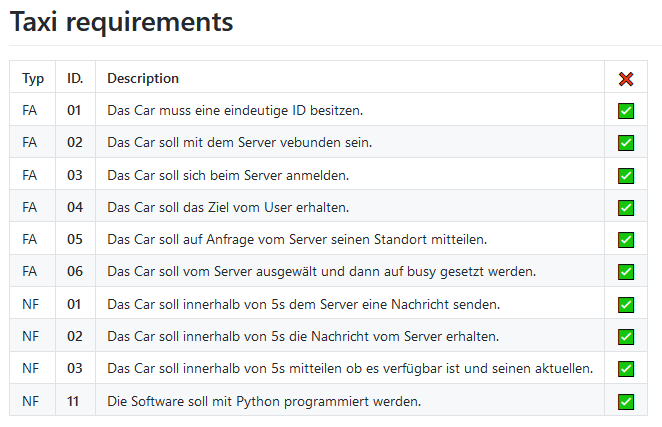
\includegraphics[width=0.48\textwidth]{Bsp_requirments.png}
     \caption{Requirments}
\end{figure}

\subsection{Use-Case}

Der Nächste Schritt im Projekt, ist aus dem gesammelten Informationen der Requirements, Use-Case Diagramme für jeden Client zu erstellen.
Use-Case Diagramme verdeutlichen die Aufgaben und Verbindungen zwischen den einzelnen Clients.

Vorab Registrieren sich alle Clients beim Server, so ist der Server mit jedem Client verbunden. Nun bekommt der Server eine Message vom User, 'request car'.

Folgend wird 'select closest car' vom Server durchgeführt und dem nächsten gelegenen Car mitgeteilt, das eine anfragende vom User eingegangen ist. Zudem sind in der Message die Koordinaten des Users enthalten, woraufhin das Car zu diesem Standort fährt.

Der Server setzt das bestellte Car auf Busy, 'change car status'.
Danach erhält das Car eine Message vom User mit dem gewünschten Zielort und bringt ihn dort hin. Am Zielort setzt der User dann das Car beim Server wieder auf free. Zum Schluss erfragt der Server den neuen Standort des Cars und schließt die Handlung damit ab.


\begin{figure}[htbp] 
  \centering
     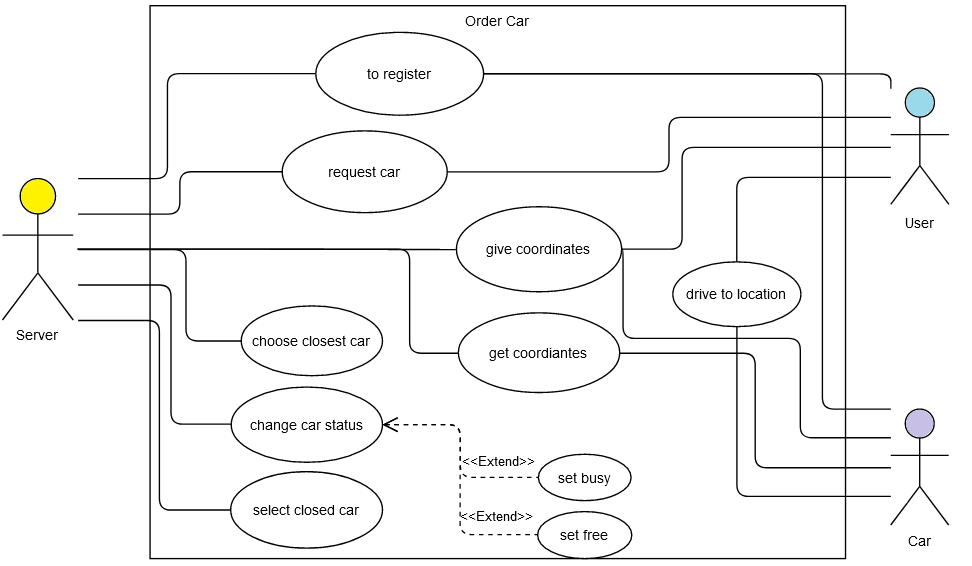
\includegraphics[width=0.48\textwidth]{Use-Case_Server.png}
     \caption{Use-Case}
\end{figure}

\subsection{Klassendiagramm}


\begin{figure}[htbp] 
  \centering
     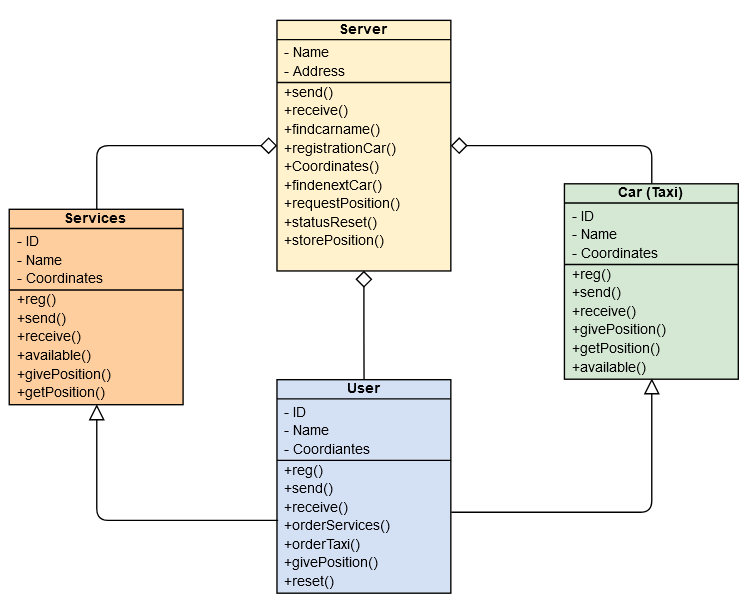
\includegraphics[width=0.48\textwidth]{Class_diagramm.png}
     \caption{Use-Case}
\end{figure}

\section{TaxiCode}

Die Aufgabe des Taxis ist es über den MQTT Server mit dem Server und dem User zu kommunizieren.
 
Über die erhaltenen Messages fährt das Taxi zum User und bringt ihn zu seinem Zielort.

Der erste Schritt vom Taxi ist, sich beim Server mit seinem Namen zu registrieren. 

Folgend weißt der Server dann dem Taxi seine ID zu.

\begin{lstlisting} 

data = {
	"id": "register", 
	"name": name,
	"coordinates": coor
    }
    
\end{lstlisting}



Daraufhin erhält das Taxi eine Message vom Server, dass ein User ein Taxi bestellt hat. 
Nun liest das Taxi die Koordinaten vom User aus. 

\begin{lstlisting} 
        data = {
        "id":id,
        "msg": "Arrival",
        "coordinates": js['coordinates']
        }
\end{lstlisting}



Mit den erhaltenden Koordinaten, weiß das Taxi an welcher Stelle sich der User befindet und fährt zu seiner aktuellen Position.
Am Zielort angekommen, wartet das Taxi auf die neue Message vom User, mit seinem neuen Zielort.


\begin{lstlisting} 
        data ={
        "id":id,
        "msg": "Arrival at destination",
        "coordinates": js['destination']
        }
\end{lstlisting}



Zum Schluss erhält das Taxi eine Anfrage vom Server, mit seiner neuen Position und sendet diese dann zum Server.

\begin{lstlisting} 
data={
        "id":id,
        "name":name,
        "coordinates":coor
        }
        send(json.dumps(data),
        "hshl/mqtt_exercise/set_position")

\end{lstlisting}


For papers published in translation journals, please give the English 
citation first, followed by the original foreign-language citation \cite{b6}.

\begin{thebibliography}{00}
\bibitem{b1} G. Eason, B. Noble, and I. N. Sneddon, ``On certain integrals of Lipschitz-Hankel type involving products of Bessel functions,'' Phil. Trans. Roy. Soc. London, vol. A247, pp. 529--551, April 1955.
\bibitem{b2} J. Clerk Maxwell, A Treatise on Electricity and Magnetism, 3rd ed., vol. 2. Oxford: Clarendon, 1892, pp.68--73.
\bibitem{b3} I. S. Jacobs and C. P. Bean, ``Fine particles, thin films and exchange anisotropy,'' in Magnetism, vol. III, G. T. Rado and H. Suhl, Eds. New York: Academic, 1963, pp. 271--350.
\bibitem{b4} K. Elissa, ``Title of paper if known,'' unpublished.
\bibitem{b5} R. Nicole, ``Title of paper with only first word capitalized,'' J. Name Stand. Abbrev., in press.
\bibitem{b6} Y. Yorozu, M. Hirano, K. Oka, and Y. Tagawa, ``Electron spectroscopy studies on magneto-optical media and plastic substrate interface,'' IEEE Transl. J. Magn. Japan, vol. 2, pp. 740--741, August 1987 [Digests 9th Annual Conf. Magnetics Japan, p. 301, 1982].
\bibitem{b7} M. Young, The Technical Writer's Handbook. Mill Valley, CA: University Science, 1989.
\end{thebibliography}
\vspace{12pt}
\color{red}
IEEE conference templates contain guidance text for composing and formatting conference papers. Please ensure that all template text is removed from your conference paper prior to submission to the conference. Failure to remove the template text from your paper may result in your paper not being published.

\end{document}
